%!TEX TS-program = xelatex
%!TEX encoding = UTF-8 Unicode

\documentclass[12pt]{scrartcl}

% JASIST Guidelines: http://onlinelibrary.wiley.com/journal/10.1002/(ISSN)1532-2890/homepage/ForAuthors.html

% ------
% Fonts and typesetting settings
\usepackage[sc]{mathpazo}
\usepackage[T1]{fontenc}
\linespread{1.05} % Palatino needs more space between lines
\usepackage{microtype}

% ------
% Page layout
\usepackage[hmarginratio=1:1,top=32mm,columnsep=20pt]{geometry}
\usepackage[font=it]{caption}
\usepackage{paralist}
\usepackage{multicol}

% ------
% Abstract
\usepackage{abstract}
	\renewcommand{\abstractnamefont}{\normalfont\bfseries}
	\renewcommand{\abstracttextfont}{\normalfont\small\itshape}

% ------
% Titling (section/subsection)
\usepackage{titlesec}
\renewcommand\thesection{\Roman{section}}
\titleformat{\section}[block]{\large\scshape\centering}{\thesection.}{1em}{}

% ------
% Header/footer
\usepackage{fancyhdr}
	\pagestyle{fancy}
	\fancyhead{}
	\fancyfoot[RO]{Journal paper Template $\bullet$ April 2012 $\bullet$ Vol. XXI, No. 1}
	%TODO: fix collision with page number.

% ------
% Bibliography
\usepackage[longnamesfirst,comma,authoryear]{natbib}
% Note: APA format.  Use \citep{citekey} for (Author Year) and \citet{citekey} for Author (Year)
% More here: http://merkel.zoneo.net/Latex/natbib.php

% ------
% Figures.  
% Custom environment to work in multicolumn
\newenvironment{Figure}
  {\par\medskip\noindent\minipage{\linewidth}}
  {\endminipage\par\medskip}
\usepackage{graphicx}


% ------
% Maketitle metadata
% \title{\vspace{-15mm}%
% 	\fontsize{24pt}{10pt}\selectfont
% 	\textbf{Long Titles Look More Impressive Than Short Ones}
% 	}	
% \author{%
% 	\large
% 	\textsc{Jonathan S. Doe}\thanks{THankd to/affiliation} \\[2mm]
% 	\normalsize	University of Technology, Delft \\
% 	\normalsize	\href{mailto:frits@howtoTeX.com}{frits@howtoTeX.com}
% 	\vspace{-5mm}
% 	}
% \date{}

\title{title}
\author{author}

%%%%%%%%%%%%%%%%%%%%%%%%
\begin{document}
%
% Note about quotes: There are no smartquotes in LaTeX. 
% Use `' or ``'', not '' "".
% Also, you must escape most special characters: \& \$ \%
%

\maketitle
\thispagestyle{fancy}

\begin{multicols}{2}

\begin{abstract}
We surveyed 101 producers and consumers of phylogenetic data to determine their perceptions of the ease and importance of providing phylogenetic metadata when archiving results in a data repository.  We found that producers labeled a majority of metadata types as easy to produce, suggesting that the production of metadata is not as much of a barrier to data sharing and metadata quality in this field as was previously thought.  
These results suggest that computational sciences such as phylogenetics may have different barriers to data sharing, reuse, and quality than other sciences.  As more sciences use computational methods and reuse data, understanding these new needs will be critical to the effective functioning of data repositories and development of data management policies.
\end{abstract}


\section{Introduction}
Phylogenetics is the science of deriving probable evolutionary relaitonships from characteristics of clades (i.e. groups of organisms of varying size).  
The Open Tree of Life project %TODO: cite.  Which paper?
is a multi-institutional, NSF-funded phylogenetic synthesis project.  It is motivated by the fact that, despite many years of study, there still doesn't exist a comprehensive account of our knowledge of the evolutionary relationships of all known species.  The project seeks to collect and synthesize these trees, beginning with two example taxa.
This project is of interest to those of us studying the archiving, sharing, and reuse of data for several reasons.  First, as a large synthesis project, it is exemplary of the kind of large scale, distrubuted scientific data projects that are increasingly shaping the availability of research data in several fields... %TODO: see, e.g. cite, cite
Second, phylogenetics is a prime example of a computational science, where experements are performed by computation (\textit{in silico}) as opposed to in physical laboratories (\textit{in vivo}).  Phylogenetics is also notable in that much of the data used to produce trees is itself the result of computations (e.g. genetic sequence alignments).  This adds an added layer of complexity to the field's data reuse that presages a coming trend in science: the expansion of secondary computational anayses of computational analysis.  In this way, examinations of this discipline are likely to yeild insights robust to coming changes in science.


Phylogenetics as a field also has a history of direct involvement in its own informatics (i.e. phyloinformatics). %TODO: e.g. cite, cite
Cite these:
\begin{itemize}
	item Metadata quality
	item Minimum information standards \citep{Leebens-Mack2006}
	item Data formats \citep{Vos2012}
	item Data reuse
\end{itemize}

In this study we are most interested in examining scientists' perceptions of the ease and importance of metadata, to understand how these might shed light on data sharing and reuse in the field
User-centered evaluation

\subsection{Research Questions}
There are two primary research questions in this study.  
\begin{compactitem}
	\item[Q1] What perceptions do producers of phylogenetic trees have regarding the ease of providing metadata?
	\item[Q2] What perceptions do consumers of phylogenetic trees have regarding the importance of metadata for evaluating and reusing trees from repositories?
\end{compactitem}
Regarding Q1, previous studies such as \citet{Stoltzfus2012} indicating that phylogenetic data sharing was as low as 4\%, and \citet{Drew2013} estimate that only 64\% of these have metadata sufficient for reuse. This led us to believe that producers' attitudes would be biased against metadata production and could be an explanation for low data submission rates and poor metadata quality.  Consquently, the specific hypothesis we developed to test Q1 can be stated thus:
\begin{compactitem}
	\item[H1] Producers perceive most phylogenetic metadata types as difficult to produce
\end{compactitem}
If true, this hypothesis would suggest that increasing the ease of metadata production and data submission to repositories is the path forward for improving the quantity and quality of phylogenetic data shared and its associated metadata.
Regarding Q2, previous studies...%TODO: cite previous studies on phylogenetic reuse .
In general, we assumed that consumers of trees would view a majority of metadata categories as critical to reuse.  \citet{Stoltzfus2012} found 21 of 40 articles in a sample reused genetic sequences.  While the rate of reuse of phylogenies was much lower, it's worth noting that fully 5 of the 40 studies reused trees from the same, high quality data source, the phylogeny of plant taxa maintained by the Angiosperm Phylogeny Group. %TODO: cite
This suggests that the availability of high quality, well annotated phylogenetic data will increase reuse.  Our hypothesis regarding Q2 is thus:
\begin{compactitem}
	\item[H2] Consumers will perceive a majority of metadata types as critical to reuse
\end{compactitem}
If true, this hypothesis would explain the observed low rate of phylogenetic data reuse.

\section{Related Literature}

Phylogenetics

Science more broadly (Angela)

Edge: Computational Science
in silico vs in vivo
automated provenance

Methods etc
User-centered evaluation

\begin{compactitem}
  \item asdf
\end{compactitem}

\section{Methods}
%Karen's section

\section{Results}
Figure~\ref{label}
\begin{Figure}
	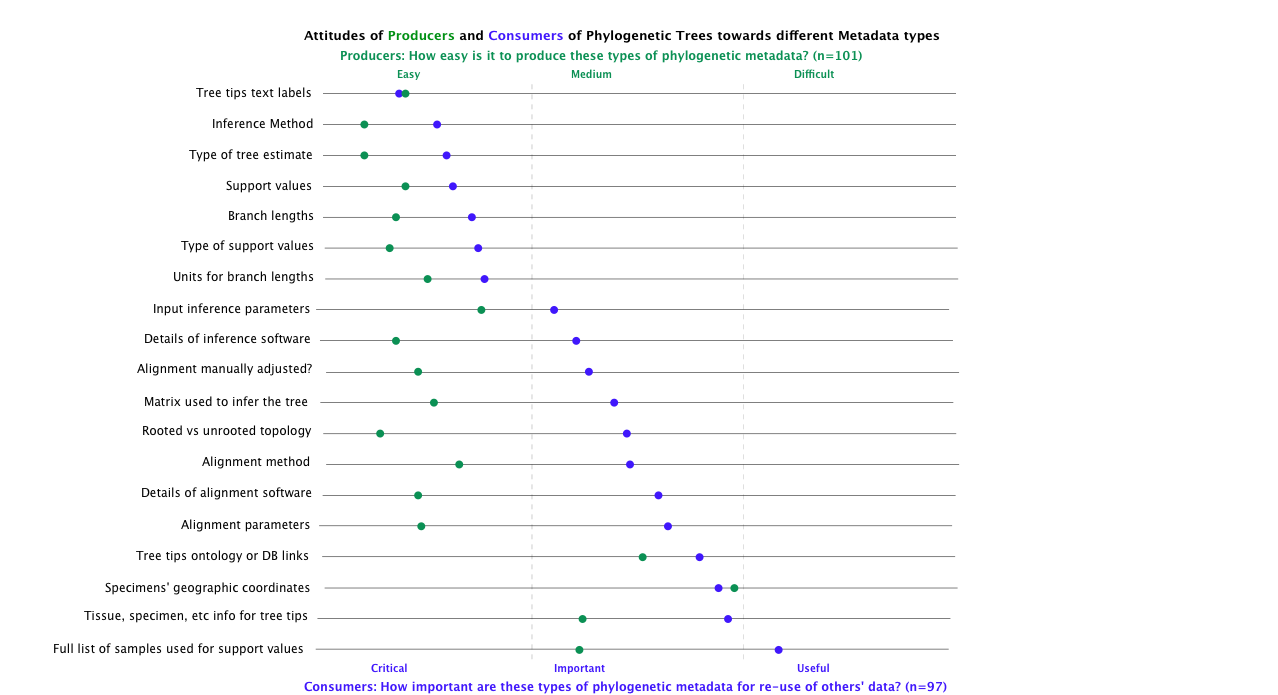
\includegraphics[width=3in]{rasters/OTOL graph - wide.png}
	\captionof{figure}{Caption}
	\label{label}
\end{Figure}

\section{Discussion}
We found evidence that both of our hypotheses were false. 

H1: producers reported that much of the metadata we asked about was produced automatically by the programs that they use.

H2: Consumers seemed confident that they could effectively evaluate phylogenetic data with relativelty few metadata types

\subsection{Preliminary Verification}
Our results suggest that the next step in confirming these results will be to investigate the actual data and metadata in common repositories.  To inform our discussion, we undertook a small, uncontrolled examination of XX%TODO: fill in
studies in data repository Dryad %TODO: cite
Of these, we found... %TODO: table here.

\subsection{Limitations}
There are several limitations of our study that suggest caution in interpreting the results as we have here.  First, the low n (=101)

\section{Conclusion}

We surveyed 101 producers and consumers of phylogenetic data to determine their perceptions of the ease and importance of providing phylogenetic metadata when archiving results in a data repository.  We found that producers labeled a majority of metadata types as easy to produce, suggesting that the production of metadata is not as much of a barrier to data sharing and metadata quality in this field as was previously thought.  
%TODO: elaborate on Conusmers
These results suggest that computational sciences such as phylogenetics may have different barriers to data sharing, reuse, and quality than other sciences.  As more sciences use computational methods and reuse data, understanding these new needs will be critical to the effective functioning of data repositories and development of data management policies.
%Bibliography note: this is keyed to Elliott's Mendeley bib dump, so pass any added references to me for inclusion.  I'll export a purposive .bib file once we're done.
\bibliographystyle{apa}
\bibliography{BibTex}

\end{multicols}

\end{document}
